% This is LLNCS.DEM the demonstration file of
% the LaTeX macro package from Springer-Verlag
% for Lecture Notes in Computer Science,
% version 2.4 for LaTeX2e as of 16. April 2010
%
\documentclass{llncs}
%
\usepackage{makeidx}  % allows for indexgeneration
\usepackage{fancyvrb}
\usepackage{graphicx}
\usepackage{subfig}
\usepackage{xspace}
\usepackage{multirow}
\usepackage{wrapfig}
\usepackage[]{algorithm2e}

\newlength{\figcapspace}
\setlength{\figcapspace}{-3ex plus 2pt minus 3pt}
\newcommand{\scap}[2]{\vspace*{\figcapspace}\caption{\sl #2}\label{#1}}

\newlength{\figtopspace}
\newlength{\figbottomspace}
\setlength{\figtopspace}{-2pt}
\setlength{\figbottomspace}{-2pt plus 2pt minus 1pt}

\newlength{\tabtopspace}
\newlength{\tabbottomspace}
\setlength{\tabtopspace}{-1ex}
\setlength{\tabbottomspace}{-1ex plus 2pt minus 2pt}

\setcounter{topnumber}{4}
\setcounter{bottomnumber}{4}
\renewcommand{\topfraction}{.9}
\renewcommand{\bottomfraction}{.9}
\setcounter{totalnumber}{6}
\renewcommand{\floatpagefraction}{.9}
\renewcommand{\dblfloatpagefraction}{.9}
\renewcommand{\dbltopfraction}{.9}
\setcounter{dbltopnumber}{4}
\renewcommand{\textfraction}{.1}

\newenvironment{topfig}{\begin{figure}[tb]
\vspace{\figtopspace}}{\vspace{\figbottomspace}
\end{figure}}

\newenvironment{dblfig}{\begin{figure*}[tb]
\vspace{\figtopspace}}{\vspace*{\figbottomspace}
\end{figure*}}

\newenvironment{toptab}{\begin{table}[tb]
\vspace{\tabtopspace}}{\vspace{\tabbottomspace}
\end{table}}
\newenvironment{dbltab}{\begin{table*}[tb]
\vspace{\tabtopspace}}{\vspace{\tabbottomspace}
\end{table*}}

\newcommand{\sectref}[1]{Sect.~\ref{#1}\xspace}

\newenvironment{tightdescription}%
        {\begin{list}{}{%
                \setlength{\itemsep}{0pt}%
                \setlength{\topsep}{0pt}%
                \setlength{\parskip}{0pt}%
                \setlength{\parsep}{0pt}%
                %\setlength{\leftmargin}{-1mm}%
        }}%
        {\end{list}}

\newenvironment{tightitemize}%
        {\begin{list}{$\bullet$}{%
                \setlength{\itemsep}{0ex}\setlength{\topsep}{0pt}%
                \setlength{\parskip}{0pt}\setlength{\parsep}{0pt}%
                \setlength{\labelwidth}{0.25cm}%
                \setlength{\leftmargin}{0cm}\addtolength{\leftmargin}{\labelwidth}\addtolength{\leftmargin}{\labelsep}%
        }}%
        {\end{list}}

%
\usepackage{latexsym}
\usepackage{amssymb}            % for \multimap (-o)
\usepackage{stmaryrd}           % for \binampersand (&), \bindnasrepma (\paar)

\newcommand{\m}[1]{\mathsf{#1}}
\newcommand{\f}[1]{\framebox{#1}}

\newcommand{\eph}{\mathit{eph}}
\newcommand{\pers}{\mathit{pers}}
\newcommand{\um}[1]{\underline{\m{#1}}}

\newcommand{\seq}{\vdash}
\newcommand{\semi}{\mathrel{;}}
\newcommand{\lequiv}{\mathrel{\dashv\vdash}}

% symbols of linear logic
\newcommand{\lolli}{\multimap}
\newcommand{\tensor}{\otimes}
\newcommand{\with}{\mathbin{\binampersand}}
\newcommand{\paar}{\mathbin{\bindnasrepma}}
\newcommand{\one}{\mathbf{1}}
\newcommand{\zero}{\mathbf{0}}
\newcommand{\bang}{{!}}
\newcommand{\whynot}{{?}}
\newcommand{\bilolli}{\mathrel{\raisebox{1pt}{\ensuremath{\scriptstyle\circ}}{\lolli}}}
% \oplus, \top, \bot


\begin{document}
\newcommand{\cmu}{\ensuremath{^\dag}}
\newcommand{\fcup}{\ensuremath{^\ddag}}
\pagestyle{headings}  % switches on printing of running heads
\addtocmark{On Compiling Linear Logic Programs}
\mainmatter              % start of the contributions
%
\title{On Compiling Linear Logic Programs with Comprehensions, Aggregates and Rule
Priorities}
%
\titlerunning{Compiling Linear Logic Programs}
\author{Flavio Cruz\inst{1}\inst{2} \and Ricardo Rocha\inst{2}}

\institute{Carnegie Mellon University, Pittsburgh, PA 15213, USA\\
\email{fmfernan@cs.cmu.edu}
\and
CRACS \& INESC TEC and Faculty of Sciences, University of Porto\\
Rua do Campo Alegre, 1021/1055, 4169-007 Porto, Portugal\\
\email{\{flavioc, ricroc\}@dcc.fc.up.pt}}

\maketitle

\begin{abstract}
Forward-chaining linear logic programs are challenging to implement efficiently
because facts are asserted and retracted frequently.  Implementation is made
more difficult with the introduction of useful features such as rule priorities,
which are used to specify the order of rule inference, and comprehensions and
aggregates, which are mechanisms that make data iteration and gathering more intuitive.  In
this paper, we describe a compilation scheme for transforming linear logic
programs enhanched with those features into efficient C++ code. Our experimental
results show that compiled logic programs are less than one order of magnitude
slower than hand-written C programs and much faster than interpreted
languages such as Python.

\end{abstract}

\section{Introduction}
Linear Meld~(LM) is a linear logic programming language aimed for the parallel
implementation of graph-based algorithms~\cite{cruz-iclp14}.  LM is a high-level
declarative language that offers a concise and expressive framework to define
graph based algorithms that are provably correct.  LM has been applied to a wide
range of problems and machine learning algorithms, including: belief
propagation~\cite{Gonzalez+al:aistats09paraml}, belief propagation with residual
splash~\cite{Gonzalez+al:aistats09paraml}, PageRank, graph coloring, N-Queens,
shortest path, diameter estimation, map reduce, quick-sort, neural network
training, minimax, and many others.

Like Datalog, LM is a \emph{forward-chaining} logic programming language since
computation is driven by a set of inference rules that are used to update a
database of logical facts.  In Datalog, programs are monotonic and therefore the
database grows in size as more facts are inferred from the logical rules. In LM,
logical facts are linear and thus can be retracted when a rule is inferred. The
use of linear facts greatly increases the power of the language but also
increases the complexity of the implementation since database facts are
retracted often.

In previous work~\cite{cruz-ppdp14}, we have described the implementation of the
LM virtual machine, including its data structures and how programs are
paralellized. In this paper, we describe our compilation strategy
and how we have refitted the runtime system to allow stand-alone compilation of
programs by transforming logical rules into C++ code.

Our goal was to reduce the overhead of executing interpreted byte code and
better understand the effectiveness and limitations of the compilation scheme.
We present an algorithm that compiles logical rules, including comprehensions
and aggregates, into efficient iterator-based C++ code.  The compiler supports
rule priorities, allowing the programmer to order rules based on their priority
of inference. To the best of our knowledge, this is the first available
compilation strategy for a linear logic language that supports these 3 features
combined. The contributions of this paper are then three-fold: (1) a novel
algorithm to compile prioritized linear logic rules with aggregates and
comprehensions; (2) the interplay between the database layout and compiled code;
and (3) comparison and analysis of our compilation with hand-written C programs
and interpreted code.  Experimental results show that our compiled programs are
only 2 to 7 times slower than hand-written C programs.

The remainder of the paper is organized as follows. First, we briefly introduce
the LM language. Next, we present an overview of the runtime support available
to compiled rules and we discuss our contributions which include the algorithm
for compiling rules into efficient iterator-based C++ code, and related work. We
then present experimental results comparing our compiled programs with the old
implementation and with hand-written C programs.  The paper finishes with some
conclusions.


\section{Linear Meld}
\newcommand{\mytt}[1]{\texttt{#1}}
\newcommand{\comprehension}[3]{\{ \; #1; \; #2; \; #3 \; \}}
\newcommand{\aggregate}[6]{[\; #1 \Rightarrow #2; \; #3; \; #4; \; #5; \; #6 \;]}

LM is a forward-chaining linear logic programming language that allows logical
facts to be asserted and retracted in a structured fashion. LM is suitable to
write parallel graph-based algorithms using implicit parallelism.
A LM program can be seen as a graph of nodes, where each node contains a
database of logical facts. The program is written as a set of inference rules
that apply over the logical facts of a node. When rules are applied, facts are
asserted or retracted from the node database.

LM rules have the form \mytt{a(X), b(Y) -o c(X, Y)} and can be read as follows:
if fact \mytt{a(X)} and fact \mytt{b(Y)} exist in the database then fact \mytt{c(X,
      Y)} is added to the database. The expression \mytt{a(X), b(Y)} is called
the \emph{body} of the rule and \mytt{c(X, Y)} is called the \emph{head} of the rule.
A fact is a predicate, e.g., \mytt{a}, \mytt{b} or \mytt{c}, and its associated
tuple of values, e.g., the concrete values of \mytt{X} and \mytt{Y}. Since LM
uses linear logic as its foundation, we distinguish between \emph{linear} and
\emph{persistent facts}. Linear facts are consumed (deleted) during the process of deriving
a rule, while persistent facts are not.  Program execution starts by adding the
initial facts (called the axioms) to the database. Next, rules are recursively
applied and the database is updated by adding new facts or deleting facts used
during rule derivation.  When no more rules are applicable, the program
terminates. Rules have a defined priority (their position in the source file)
and higher priority rules are fired first. If a new fact is derived and there is
a set of applicable rules to be fired, the higher priority rule is 
selected before the others.

To make these ideas concrete, Fig.~\ref{code:shortest_path_program} presents
a simple example for the single source shortest path~(SSSP) program.
The program computes
the shortest distance from node \mytt{@1} to all other nodes in the
graph.
The SSSP program starts (lines 1-3) with the declaration of the predicates.
Predicates specify the facts used in the program. The first predicate,
\mytt{edge}, is a persistent predicate that describes the
relationship between the nodes of the graph, where the third argument
represents the weight of the edge (the \mytt{route} modifier
informs the compiler that the \mytt{edge} predicate
determines the structure of the graph).  The predicates
\mytt{shortest} and \mytt{relax} are specified as linear facts
and thus are deleted when deriving new facts.
Every node has a \mytt{shortest} fact that is improved with
new \mytt{relax} facts.  Lines 5-9 declare the axioms of the
program: \mytt{edge} facts describe the graph; \mytt{shortest(A,
+00, [])} is the initial shortest distance (infinity) for all
nodes; and \mytt{relax(@1, 0, [@1])} starts the algorithm by
setting the distance from \mytt{@1} to \mytt{@1} to be 0.

\begin{topfig}
\scriptsize\begin{Verbatim}[numbers=left]
type route edge(node, node, int).
type linear shortest(node, int, list int).
type linear relax(node, int, list int).

!edge(@1, @2, 3). !edge(@1, @3, 1).
!edge(@3, @2, 1). !edge(@3, @4, 5).
!edge(@2, @4, 1).
shortest(A, +00, []).
relax(@1, 0, [@1]).

shortest(A, D1, P1), D1 > D2, relax(A, D2, P2)
   -o shortest(A, D2, P2),
      {B, W | !edge(A, B, W) |
         relax(B, D2 + W, P2 ++ [B])}.

shortest(A, D1, P1), D1 <= D2, relax(A, D2, P2)
   -o shortest(A, D1, P1).
\end{Verbatim}
\caption{Single Source Shortest Path program code.}
\label{code:shortest_path_program}
\end{topfig}

The first rule of the program (lines 11-14) reads as following: if the current
\mytt{shortest} path \mytt{P1} with distance \mytt{D1} is larger
than a new path \mytt{relax} with distance \mytt{D2}, then replace the
current shortest path with \mytt{D2}, delete the new \mytt{relax} path and
propagate new paths to the neighbors (lines 13-14) using a \emph{comprehension}.
The comprehension iterates over the edges of node \mytt{A} and derives a new
\mytt{relax} fact for each node \mytt{B} with the distance \mytt{D2 + W},
where \mytt{W} is the weight of the edge.

The second rule of the program (lines 16-17) is read as following: if the
current shortest path \mytt{D1} is shorter than the a path \mytt{D2} then
delete the new \mytt{relax} fact and keep the current shortest path.

Figure~\ref{fig:shortest_path_program} shows a graphical representation of the
application of the SSSP program rules.

\begin{figure}[ht]
\begin{center}
  \subfloat[]{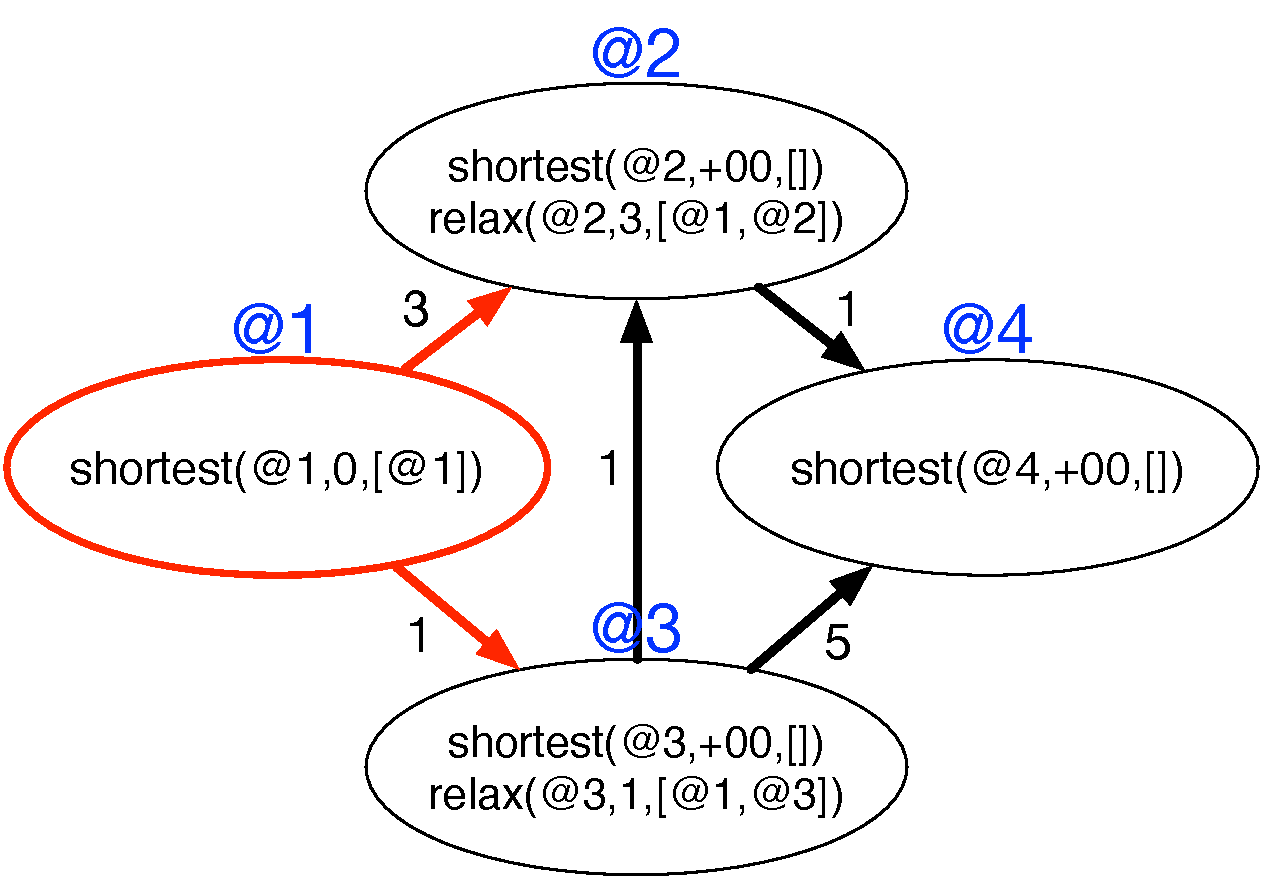
\includegraphics[width=0.3\textwidth]{figures/shortest2}}
  \hspace{0.4cm}
  \subfloat[]{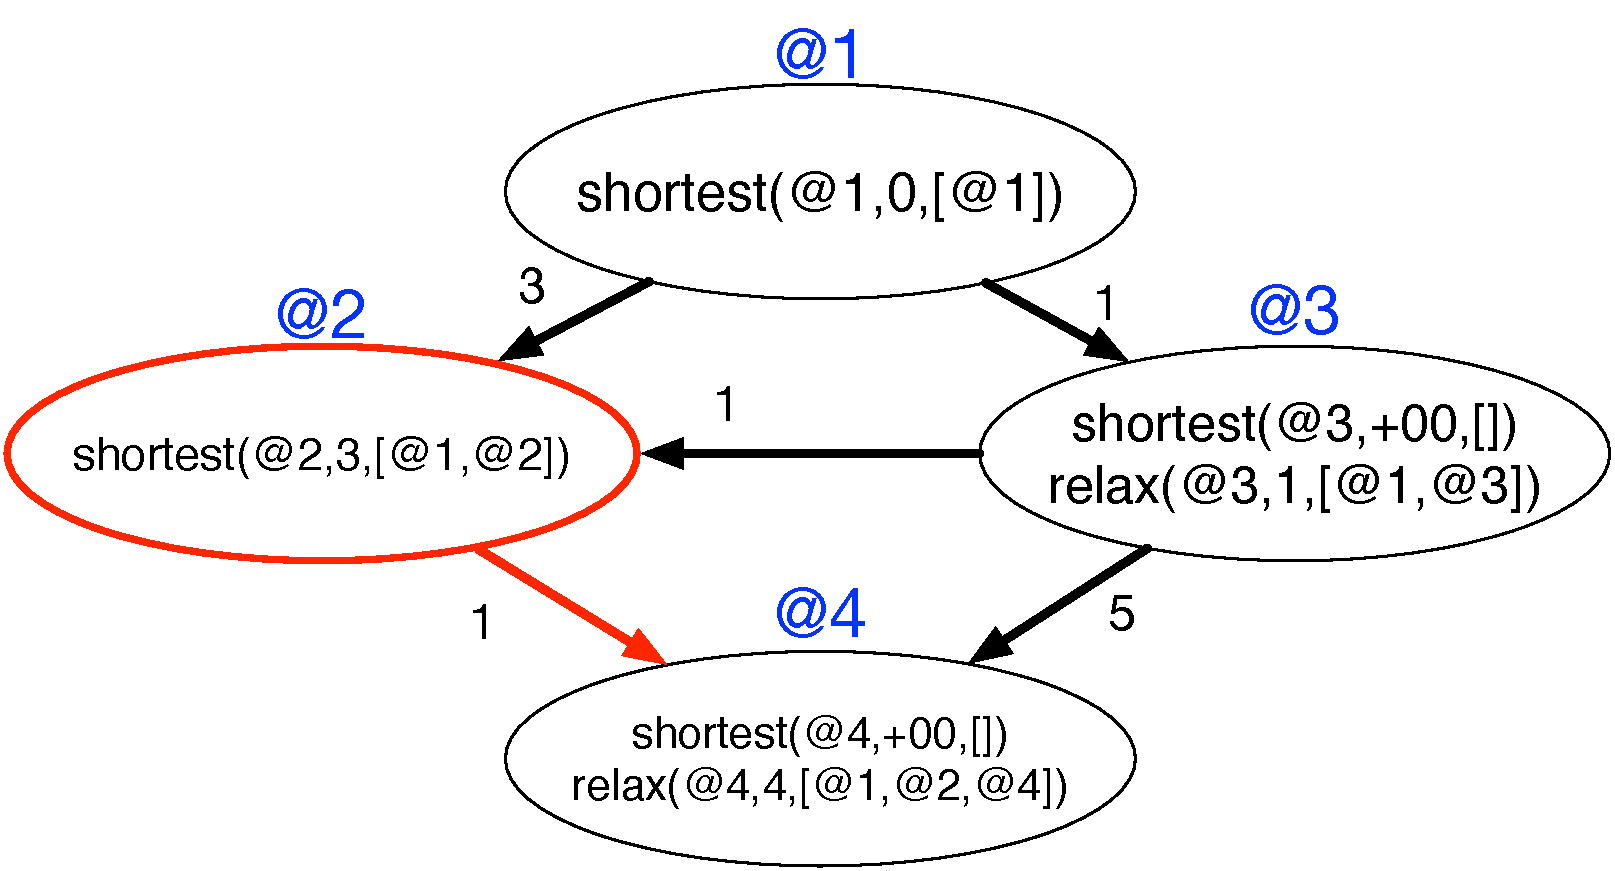
\includegraphics[width=0.3\textwidth]{figures/shortest3}}
  \hspace{0.4cm}
  \subfloat[]{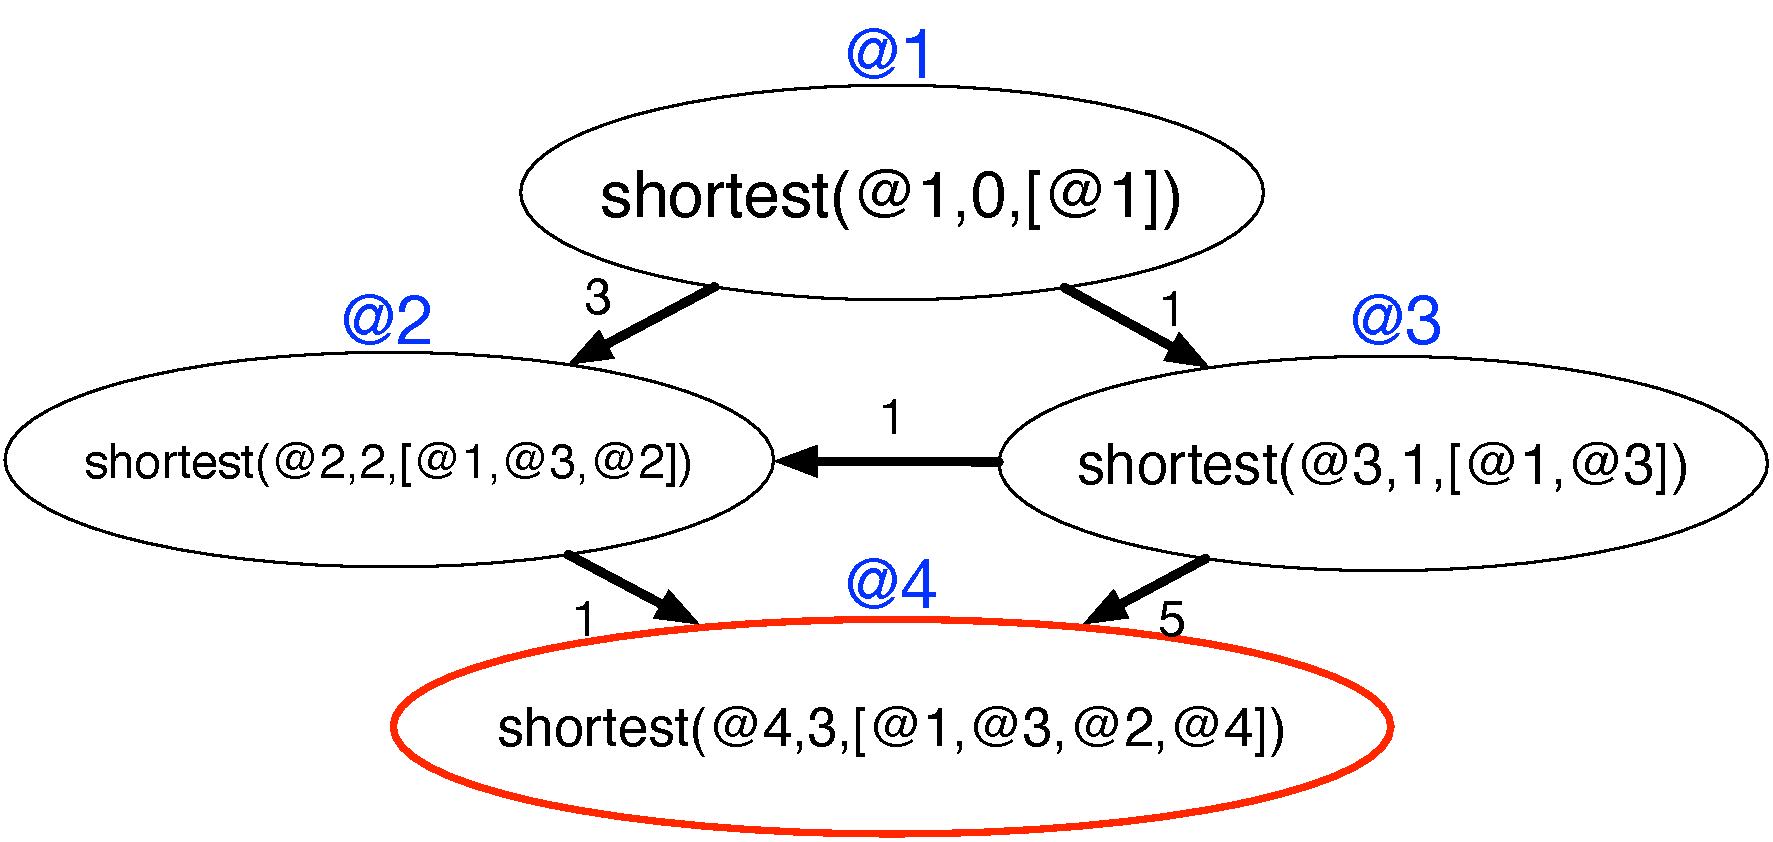
\includegraphics[width=0.3\textwidth]{figures/shortest8}}
\end{center}
\caption{Graphical representation of the SSSP program. (a) represents the
   program after propagating initial distance at node \mytt{@1}, followed by
   (b) where the first rule is applied in node \mytt{@2}. (c)
   represents the state of the final program, where all the shortest paths
   have been computed.}
\label{fig:shortest_path_program}
\end{figure}


\subsection{LM Syntax}

\begin{table}[h]
\centering
\begin{tabular}{ l l c l }
  Program & $Prog$ & $::=$ & $\Sigma, D$ \\
  List Of Rules & $\Sigma$ & $::=$ & $\cdot \; | \; \Sigma, R$\\
  Database & $D$ & $::=$ & $\Gamma; \Delta$ \\
  Rule & $R$ & $::=$ & $BE \lolli HE \; | \; \forall_{x}. R$ \\
  Body Expression & $BE$ & $::=$ & $L \; | \; P \; | \; C \; | \; BE, BE \; | \; \one$\\
  Head Expression & $HE$ & $::=$ & $L \; | \; P \; | \; HE, HE \; | \; EE \; |
  \; CE \; | \; AE \; | \; \one$\\
  
  Linear Fact & $L$ & $::=$ & $l(\hat{x})$\\
  Persistent Fact & $P$ & $::=$ & $\bang p(\hat{x})$\\
  Constraint & $C$ & $::=$ & $c(\hat{x})$ \\
  Selector Operation & $S$ & $::=$ & $\mathtt{min} \; | \; \mathtt{max} \; | \; \mathtt{random}$\\
  
  Comprehension & $CE$ & $::=$ & $\comprehension{\widehat{x}}{SB}{SH}$ \\

  Aggregate & $AE$ & $::=$ & $\aggregate{A}{y}{\widehat{x}}{SB}{SH_1}{SH_2}$ \\
  Aggregate Operation & $A$ & $::=$ & $\mathtt{min} \; | \; \mathtt{max} \; | \;
\mathtt{sum} \; | \; \mathtt{count} \; | \; \mathtt{collect}$ \\
  
  Sub-Body & $SB$ & $::=$ & $L \; | \; P \; | \; SB, SB \; | \; \exists_{x}. SB$\\
  Sub-Head & $SH$ & $::=$ & $L \; | \; P \; | \; SH, SH \; | \; \one$\\
  
  Known Linear Facts & $\Delta$ & $::=$ & $\cdot \; | \; \Delta, l(\hat{t})$ \\
  Known Persistent Facts & $\Gamma$ & $::=$ & $\cdot \; | \; \Gamma, \bang p(\hat{t})$ \\
\end{tabular}
\caption{Abstract syntax of LM.}\label{tbl:ast}
\end{table}

The abstract syntax for LM programs is presented in Table~\ref{tbl:ast}.  A LM
rule is written as $BE \lolli HE$ where $BE$ is the body and $HE$ is the head of
the rule. The body may contain linear ($L$) and persistent ($P$) \emph{fact
   expressions} and \emph{constraints} ($C$). Fact expressions instantiate facts from
   the database and contain variables as arguments that may or may not be bound
   to concrete values or to other variables.
   Variables in the body of the rule can also be used in the
   head when instantiating facts.
  
Fact constraints are essential
for matching rules since they represent database \emph{joins} and database
\emph{selects}.
While selects filter out possible combinations from the database,
body constraints ($C$) further restrict combinations by acting as guards using
small variables from fact expressions. Constraints use a small
functional language that includes mathematical
operations, boolean operations, external functions and literal values.

The head of a rule, $HE$, contains linear ($L$) and persistent ($P$) \emph{fact
   templates} which are uninstantiated facts and will derive new facts. The head
   can also have \emph{comprehensions} ($CE$) and \emph{aggregates} ($AE$). All
   those expressions may use all the variables instantiated in the body.

\subsubsection{Comprehensions} are similar to the functional programming
construct of the same name.  Comprehensions are sub-rules that are applied
for all possible combinations. In a comprehension
$\comprehension{\widehat{x}}{SB}{SH}$, $\widehat{x}$ is a list of variables,
$SB$ is the body of the comprehension and $SH$ is the head. The body $SB$ is
used to generate all possible combinations for the head $SH$, according to the
facts in the database.  An example was shown in
Fig.~\ref{code:shortest_path_program} (lines 13-14), where \mytt{\bang edge(A,
      B, W)} facts are iterated over in order to derive \texttt{relax(A, D2 + W,
         P2 ++ [B])} facts for each combination.

\subsubsection{Aggregates}
build on top of comprehensions and allow the capture of values that
appear in each combination of the sub-rules. This list of values is then
combined using one operator into a single value and then used to derive a set of
fact expressions. In the abstract syntax
$\aggregate{A}{y}{\widehat{x}}{SB}{SH_1}{SH_2}$, $A$ is the aggregate operation,
$\widehat{x}$ is the list of variables introduced in $BE$ and $SH_1$ and $y$ is
the variable in the body $SB$ that represents the values to be aggregated using
$A$. Like comprehensions, we use $\widehat{x}$ to try all the combinations of
$SB$, but, in addition to deriving $SH_1$ for each combination, we aggregate the
values represented by $y$ into a new $y$ variable that is used inside the head
$SH_2$.  LM provides several aggregate operations, including the \texttt{min}
(minimum value), \texttt{max} (maximum value), \texttt{sum} (add all numbers),
\texttt{count} (count combinations) and \texttt{collect} (collect items into a
list). Consider, for example, the following rule:

\begin{Verbatim}[fontsize=\scriptsize]
update(A), pagerank(A, OldRank)
      -o [sum => V | B | neighbor-pagerank(A, B, V) |
            neighbor-pagerank(A, B, V) |
            pagerank(A, damp/P + (1.0 - damp) * V)].
\end{Verbatim}

The rule uses an aggregate to accumulate the sum of the
neighbor's pageranks into a single value. This value is then assigned to a new
\texttt{pagerank} fact by computing \texttt{damp/P + (1.0 - damp)*V}, where
\texttt{V} is the aggregate value. \texttt{V} is the result of adding all the
values in \texttt{neighbor-pagerank(A, B, V)} facts.





\section{Supporting Runtime and Database Data Structures}\label{sec:data_structures}

In this section, we review the supporting runtime that is used by the compiler.
We focus mostly on the structure of the nodes since inference rules are compiled
from the point of view of the node data structure.

Figure~\ref{fig:node} presents the layout of the node data structures.  Each
node of the graph stores 4 main data structures: (1) the \emph{rule matching
   engine}; (2) a \emph{fact buffer} for storing incoming and temporary facts;
(3) the \emph{database of linear facts}; and (4) the \emph{database of
   persistent facts}.

The rule engine maintains a simplified view of the two fact databases and
efficiently decides which rules need to be executed. For instance, if a rule $r$
needs facts \texttt{a} and \texttt{b} to be applied and the database already
contains \texttt{a} facts, once a \texttt{b} fact is derived, the rule engine
schedules $r$ to be executed. The compiler is responsible for the code that is
executed when a rule is scheduled.  A compiled rule contains instructions to
search and match facts from the database and to derive new facts when the body
of the rule is successfully matched.

In this context, the organization of the database structures is critical because
linear facts can be retracted and asserted frequently. This means that the
database needs to allow fast insertions and deletions but also needs to have
reasonably fast mechanisms for lookup. The database of facts is partitioned by
predicate, therefore, each predicate can have its own data structure depending
on the patterns of access for that particular predicate. Linear facts are stored
using the following data structures:

\begin{wrapfigure}{r}{0.5\textwidth}
\vspace{-1cm}
\begin{center}
   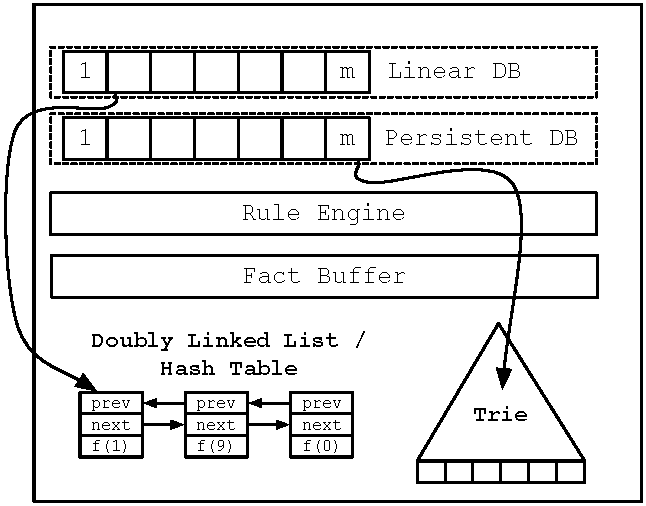
\includegraphics[width=0.5\textwidth]{figures/overview.pdf}
\end{center}
\caption{Node data structures.}
\label{fig:node}
\vspace{-2cm}
\end{wrapfigure}


\begin{itemize}

\item \emph{Doubly-Linked List Data Structures}. Each linear fact is a node of
   the linked list. Allows constant $\mathcal{O}(1)$ insertion and deletion of
   facts given the pointer of the target node. Although lookup operations take
   linear time, this is not critical since most predicates tend to have a small
   number of facts.

\item \emph{Hash Table Data Structures}. For predicates with many facts we use
   hash tables. Hash tables are more efficient for repetitive lookup
   operations using a specific argument (i.e., searching for facts with a
   concrete value) and build upon lists by hashing facts using a
   specific argument and then using separate chaining with doubly-linked lists
   for collision resolution. Hash tables are, on average, $\mathcal{O}(1)$ for
   insertion, deletion and lookup, however they require more memory.

\end{itemize}

For persistent tuples, we use \emph{Trie Data Structures}, which are trees where
facts are indexed by a common prefix. Since persistent facts are never deleted,
it's not expensive to index facts by a common prefix, which also tends to save
memory in the long run.



\section{Compiling Rules}\label{sec:compile}

In this section, we present the main algorithm of the compiler, that turns
inference rules into C++ code, and we discuss the key optimizations for
efficient code execution.

\subsection{Ordinary Rules}\label{sec:compile}

After an inference rule is compiled, it must respect the \emph{fact constraints}
(facts must exist in the database) and the \emph{join constraints} that can be
represented by variable constraints and/or boolean expressions. For instance,
consider gain the second rule of the SSSP program presented in
Fig.~\ref{code:shortest_path_program}:

\begin{Verbatim}[fontsize=\scriptsize,label=example_rule]
shortest(A, D1, P1), D1 <= D2, relax(A, D2, P2)
   -o shortest(A, D1, P1).
\end{Verbatim}

The fact constraints include the facts required to trigger the rule, namely
\texttt{shortest(A, D1, P1)} and \texttt{relax(A, D2, P2)}, and the join
constraints include the expression \texttt{D1 <= D2}.

However, rules may also have other less obvious join constraints such as:

\begin{Verbatim}[fontsize=\scriptsize]
new-neighbor-pagerank(A, B, New),
neighbor-pagerank(A, B, Old)
   -o neighbor-pagerank(A, B, New).
\end{Verbatim}

where variable \texttt{B} must have the same value in both facts\footnote{Rule taken
from an asynchronous PageRank program.}.

\subsection{Iterators}

The data structures for facts presented in Section~\ref{sec:data_structures}
support the \emph{iterator} pattern. For linked lists, the iterator goes
through every fact in the list while the hash table iterator can either iterate
through the whole table or iterate through a single bucket. A bucket iterator is
in fact a linked list iterator that starts from a given argument.
For tries, while the default iterator goes through every fact in
the trie, it can be customized with a matching specification in
order to reduce search. A matching specification includes argument
assignments (e.g., argument $i = V$, where $V$ is a concrete value).

Iterators are heavily used in the compiled code. For instance, the second rule in
Fig.~\ref{code:shortest_path_program} is compiled as follows:

\begin{Verbatim}[numbers=left,fontsize=\scriptsize]
for(auto it1(linked_list("shortest").begin()); it1 != linked_list("shortest").end(); )
{
   fact *f1(*it1);
   for(auto it2(linked_list("relax").begin()); it2 != linked_list("relax").end(); )
   {
      fact *f2(*it2);

      if(f1->get_int(1) <= f2->get_int(1)) {
         fact *new_shortest(new fact("shortest"));
         new_shortest->set_int(1, f1->get_int(1));
         new_shortest->set_list(2, f1->get_list(2));

         // new fact was derived
         linked_list("shortest").push_back(new_shortest);

         // deleting facts
         it1 = linked_list("shortest").erase(it1); // remove from list
         it2 = linked_list("relax").erase(it2);
         return;
      }
      ++it2;
   }
   ++it1;
}
\end{Verbatim}


The compilation algorithm iterates through the fact expressions in the body of
the rule and creates nested loops to try all the possible combinations of facts.
For this rule, all the pairs of facts \texttt{shortest} and \texttt{relax} must
be matched until the constraint \texttt{D1 <= D2} is true. First, an iterator
for \texttt{shortest} is created that will loop through all \texttt{shortest}
facts in the list. Inside the loop, a nested iterator is created for predicate
\texttt{relax}. This inner loop includes a check for the \texttt{D1 <= D2}
constraint. If the constraint expression is true then the rule matches and a new
\texttt{shortest} fact is derived and two used linear facts are retracted by
erasing the iterators from the linked lists. Note that after the rule is
derived, the code must return since there is a higher priority rule that may be
triggered with the new \texttt{shortest} fact (see
Fig.~\ref{fig:shortest_path_program}). This enforces the priority semantics
of the language.
    
If the constraint had failed, another \texttt{relax} fact would have been tried
by incrementing \texttt{it2}. Likewise, if the current \texttt{f1} fact fails
for all \texttt{f2} facts, then the next one in the list is tried
by incrementing \texttt{it1}.

\begin{figure}
\begin{algorithm}[H]
 \KwData{Rule R1, Rules}
 \KwResult{Compiled Code}
 $FactExprs \longleftarrow FactExprsFromRule(R1)$\;
 $Constraints \longleftarrow ConstraintsFromRule(R1)$\;
 $Code \longleftarrow CreateFunctionForRule()$\;
 $Iterators \longleftarrow []$\;
 $CompiledFacts = []$\;
 \While{$FactExprs$ not empty}{
  $Fact \longleftarrow RemoveBestFactExpr(FactExprs)$\;
  $CompiledFacts.push(Fact)$\;
  $Iterator \longleftarrow Code.InsertIterator(Fact)$\;
  $Iterators.push(Iterator)$\;
  \tcc{Select constraints that are covered by CompiledFacts.}
  $NextConstraints \longleftarrow RemoveConstraints(Constraints, CompiledFacts)$\;
  $Code.InsertConstraints(NextConstraints)$\;
 }
 $HeadFacts = HeadTemplatesFromRule(R1)$\;
 \While{$HeadFacts$ not empty}{
    $Fact \longleftarrow RemoveFact(HeadFacts)$\;
    $Code.InsertDerivation(Fact)$\;
 }
 \For{$Iterator \in Iterators$}{
    \If{$IsLinear(Iterator)$}{
       $Code.InsertRemove(Iterator)$\;
    }
 }
 \tcc{Enforce rule priorities.}
 \uIf{$FactsDerivedUsedBefore(Head, Program, R1)$}{
    $Code.InsertReturn()$\;
 }
 \Else{
    $Code.InsertGoto(FirstLinear(Iterators))$\;
 }
 \Return{$Code$}
\end{algorithm}
 \caption{Compiling LM rules into C++ code.}
 \label{alg:compile_rule}
\end{figure}

Figure~\ref{alg:compile_rule} presents the algorithm for compiling rules into
C++ code.  First we split the body of the rule into fact expressions and
constraints. Fact expressions map directly to iterators while fact constraints
map to \emph{if} expressions. A possible compilation strategy is to first
compile all the fact expressions and then compile the constraints. However, this
may require unneeded database lookups since some constraints may fail early.
Therefore, our compiler introduces constraints as soon as all the variables in
the constraint are all included in the already compiled fact expressions. The
order in which fact expressions are selected for compilation does not interfer
with the correctness of the compiled code, thus our compiler selects the fact
expressions ($RemoveBestFactExpr$) by their potential to activate constraints,
therefore avoiding undesirable database lookups. If two fact
expressions have the same number of new constraints, then the
compiler always picks the persistent fact expression since
persistent facts are not deleted.

Derivation of new facts belonging to the local node implies adding the new fact
to the local node data structure. Facts that belong to other nodes are sent
using an appropriate runtime API.

\subsection{Persistence Checking}

Not all linear facts need to be deleted. For instance, in the compiled rule
above, the fact \texttt{shortest(A, D1, P1)} is re-derived in the head. Our
compiler is able to turn linear loops into persistent loops for linear facts
that are retracted and then asserted.  The rule is then compiled as follows:

\begin{Verbatim}[numbers=left,fontsize=\scriptsize]
for(auto it1(linked_list("shortest").begin()); it1 != linked_list("shortest").end(); )
{
   fact *f1(*it1);
   for(auto it2(linked_list("relax").begin()); it2 != linked_list("relax").end(); )
   {
      fact *f2(*it2);
      if(f1->get_int(1) <= f2->get_int(1)) {
         it2 = linked_list("relax").erase(it2);
         goto next;
      }
      ++it2;
next: continue;
   }
   ++it1;
}
\end{Verbatim}

In this new version of the code, only the \texttt{relax} facts are deleted,
   while the \texttt{shortest} facts remain untouched. In the SSSP program, each
   node has one \texttt{shortest} fact and this compiled code simply filters out
   the \texttt{relax} facts with the distances that are equal or greater than
   the current best distance. Note that now have a \emph{goto statement} (line
         13) that is executed when the rule is fired.  In this case, since no
   new \texttt{shortest} fact was derived, we can avoid returning to enforce
   rule priorities and we can continue to try to fire the rule as many times as
   possible.

All the rule combinations are attempted in cases where a rule does not derive
any facts or the facts derived do not appear before the rule, that is, the new
facts are only used in lower priority rules. This is specified in the final
\emph{if statement} in Fig.~\ref{alg:compile_rule}. If the rule does not return,
then we always jump to the first loop that uses linear facts. We must jump to
the first linear loop because we cannot use
the next fact from the deepest loop since we may have constraints between the
first linear loop and the deepest loop that were validated using deleted facts.

\subsection{Updating Facts}

Many inference rules retract and then derive the same predicate but with
different arguments. The compiler recognizes those cases and instead of
retracting the fact from its linked list or hash table, it updates the fact
in-place. As an example, consider the following rule:

\begin{Verbatim}[fontsize=\scriptsize]
new-neighbor-pagerank(A, B, New),
neighbor-pagerank(A, B, Old)
   -o neighbor-pagerank(A, B, New).
\end{Verbatim}

Assuming that \texttt{neighbor-pagerank} is stored in a hash table and indexed by the
second argument, the code for the rule above is as follows:

\begin{Verbatim}[numbers=left,fontsize=\scriptsize]
for(auto it1(linked_list("new-neighbor-pagerank").begin()); it1 !=
      linked_list("new-neighbor-pagerank").end(); )
{
   fact *f1(*it1);
   // hash table for neighbor-pagerank is indexed by the second argument
   // therefore we search for the bucket using the second argument of new-neighbor-pagerank
   hash_bucket bucket(hash_table("neighbor-pagerank").find(f1->get_node(1));
   for(auto it2(bucket.begin()); it2 != bucket.end(); )
   {
      fact *f2(*it2);
      if(f1->get_node(1) == f2->get_node(1)) {
         f2->set_float(2, f1->get_float(2)); // update neighbor-pagerank
         it1 = linked_list("new-neighbor-rank").erase(it1);
         goto next;
      }
      ++it2;
   }
   ++it1;
next: continue;
}
\end{Verbatim}

Note that \texttt{neighbor-pagerank} is updated using \texttt{set\_float}. The
rule also does not return since this is the highest priority rule. If there
was a higher priority rule using \texttt{neighbor-pagerank}, then the code
would have to return since an update fact represents a new fact.

\subsection{Enforcing Linearity}

We have already introduced the \emph{goto} statement as a way to avoid reusing
retracted linear facts. However, this is not enough in order to enforce
linearity of facts. Consider the following inference rule:

\begin{Verbatim}[fontsize=\scriptsize]
add(A, N1), add(A, N2) -o add(A, N1 + N2).
\end{Verbatim}

Using the standard compilation algorithm, two nested loops are created, one for
each \texttt{add} fact. However, notice that there is an implicit constraint
when creating the iterator for \texttt{add(A, N2)} since this fact cannot be the
same as the first one. That would invalidate linearity since a single linear fact would
be used to prove two linear facts. This is easily solved by adding a constraint
for the inner loop by checking if the fact pointer is the same as the first one.

\begin{Verbatim}[numbers=left,fontsize=\scriptsize]
for(auto it1(linked_list("add").begin()); it1 != linked_list("add").end(); )
{
   fact *f1(*it1);
   for(auto it2(linked_list("add").begin()); it2 != linked_list("add").end(); )
   {
      fact *f2(*it2);
      if(f1 != f2) {
         f1->set_int(1, f1->get_int(1) + f2->get_int(1));
         it2 = linked_list("add").erase(it2);
         goto next;
      }
      ++it2;
   }
   ++it1;
next: continue;
}
\end{Verbatim}

Figure~\ref{fig:update_add} presents the steps for executing this rule when the
database contains three facts. The iterators never point to the same fact.

\begin{figure}
\centering
\begin{minipage}{.5\textwidth}
  \centering
  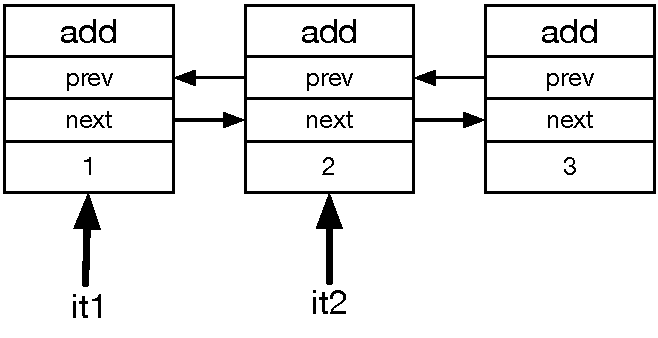
\includegraphics[width=.8\linewidth]{figures/update}
\end{minipage}%
\begin{minipage}{.5\textwidth}
  \centering
  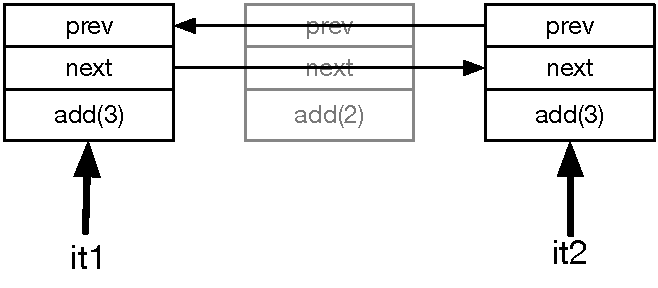
\includegraphics[width=0.8\linewidth]{figures/update2}
\end{minipage}
\begin{minipage}{.5\textwidth}
   \centering
  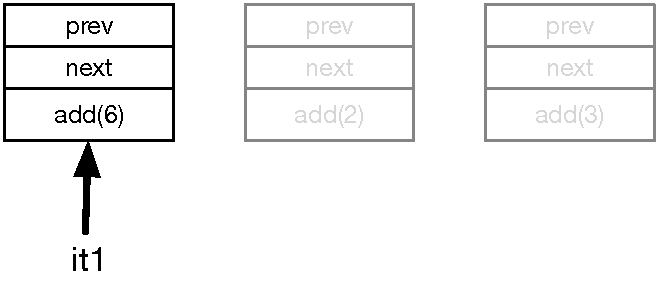
\includegraphics[width=0.8\linewidth]{figures/update3}
\end{minipage}
\caption{Executing the add rule. First, the two iterators point to
   the first and second facts and the former is updated while the latter is
   retracted. The second iterator then moves to the next fact and the first fact is
   updated again, now to the value \texttt{6}, the expected result.}
\label{fig:update_add}
\end{figure}

\subsection{Comprehensions}

Comprehensions were initially presented in the first rule of the SSSP program.

\begin{Verbatim}[fontsize=\scriptsize]
shortest(A, D1, P1), D1 > D2, relax(A, D2, P2)
   -o shortest(A, D2, P2), {B, W | !edge(A, B, W) | relax(B, D2 + W, P2 ++ [B])}.
\end{Verbatim}

The attentive reader will remember that comprehensions are sub-rules, therefore
they should be compiled like normal rules. However, they do not need to return
due to rule priorities since all the combinations of the comprehension must be
derived. However, the rule itself must return if any of its comprehensions
has derived a fact that is used by a higher priority rule.
The example rule does not need to return since it has the highest priority and the
\texttt{relax} facts derived in the comprehension are all sent to other nodes.
The code for the rule is shown below:

\begin{Verbatim}[numbers=left,fontsize=\scriptsize]
for(auto it1(linked_list("shortest").begin()); it1 != linked_list("shortest").end(); )
{
   fact *f1(*it1);
   for(auto it2(linked_list("relax").begin()); it2 != linked_list("relax").end(); )
   {
      fact *f2(*it2);
      if(f1->get_int(1) > f2->get_int(1)) {
         // comprehension code
         for(auto it3(trie("edge").begin()); it3 != trie("edge").end(); ) {
            fact *f3(*it3);
            fact *new_relax(new fact("relax"));
            new_relax->set_int(1, f2->get_int(1) + f3->get_int(2));
            new_relax->set_list(append(f2->get_list(2), list(f3->get_node(1))));
            send_fact(new_relax, f3->get_node(1));
            ++it3;
         }
         f1->set_int(1, f2->get_int(1));
         f1->set_list(2, f2->get_list(2));
         it2 = linked_list("relax").erase(it2);
         goto next;
      }
      ++it2;
   }
   ++it1;
next: continue;
}
\end{Verbatim}

Special care must be taken when the comprehension's sub-rule uses the same
predicates that are derived by the main rule.
Rule inference must be atomic in the sense that after a rule matches, the
comprehensions in the head of the rule can use the facts that were present
before the body of the rule was matched.
Consider a rule with $n$ comprehensions or aggregates, where $CB_i$ and $CH_i$
is the body and head of the comprehension/aggregate, respectively, and $H$
represents the fact templates found in the head of the rule.
The formula used by the compiler to detect conflicts between predicates is the
following:

\[
\bigcup^{n}_i[CB_i \cap H] \cup \bigcup^{n}_i [CB_i \cap \bigcup^{n}_j[CH_j]]
\]

If the result of the formula is not empty, then the compiler disables
optimizations for the conflicting predicates and derives the corresponding facts
into the fact buffer that are then added back into the database.
Fortunately, most rules in LM programs do not show conflicts and thus
can be fully optimized.

\subsection{Aggregates}

Aggregates are similar to comprehensions. They are also sub-rules but a value is
accumulated for each combination of the sub-rule. After all the combinations are
inferred, a final head term is derived with the accumulated term. Consider the following
PageRank rule:

\begin{Verbatim}[fontsize=\scriptsize]
update(A), pagerank(A, OldRank)
      -o [sum => V | B | neighbor-pagerank(A, B, V) | neighbor-pagerank(A, B, V) |
            pagerank(A, damp/P + (1.0 - damp) * V)].
\end{Verbatim}

The variable \texttt{V} is initialized to \texttt{0.0} and sums all
the PageRank values of the neighbors as seen in the code below. The aggregate
value is then used to update the second argument of the initial
\texttt{pagerank} fact.

\begin{Verbatim}[numbers=left,fontsize=\scriptsize]
for(auto it1(linked_list("pagerank").begin()); it1 != linked_list("pagerank").end(); )
{
   fact *f1(*it1);
   for(auto it2(linked_list("update").begin()); it2 != linked_list("update").end(); )
   {
      fact *f2(*it2);
      double acc(0.0); // aggregate accumulator.
      for(auto it3(linked_list("neighbor-pagerank").begin()); it3 !=
            linked_list("neighbor-pagerank").end(); ) {
         fact *f3(*it3);
         acc += f3->get_float(2);
         ++it3; // the sub-rule has no head since neighbor-pagerank is re-derived
      }
      // head of the aggregate
      f1->set_float(1, damp / P + (1.0 - damp) * V);
      goto next;
   }
   ++it1;
next: continue;
}
\end{Verbatim}


\section{Related Work}

LM shares many similarities with Constraint Handling Rules~
(CHR)~\cite{Betz:2005kx,DBLP:journals/corr/abs-1006-3039}.  CHR is a concurrent
committed-choice constraint language used to write constraint solvers. A CHR
program is a set of rules and a set of constraints.  The constraint store can be
seen as a database of facts and rules manipulate the constraint store. Many
basic optimizations used in the LM compiler such as join optimizations and the
use of different data structures for indexing facts were inspired in work done
on CHR~\cite{DBLP:journals/corr/cs-PL-0408025}.  Wuille et al.~\cite{42866} have
described a CHR to C compiler that follows some of the ideas presented here and
Koninck et al.~\cite{chrp} showed how to compile CHR programs with dynamic
priorities into Prolog. Our work distinguishes itself from these two works by
supporting a novel combination of comprehensions, aggregates and rule
priorities. Compilation of LM programs is also novel due to the implicit
parallelism of rules, allowing for programs to be parallelized.


\section{Experimental Results}\label{results}
This section presents experimental results for our compilation strategy.  We
compare the execution speed of our new compiled code against hand-written
implementations in C of the same programs. We also compare the results against
interpreted execution. Although interpreted execution uses a similar
translation, it helps us understand the limitations of the compilation scheme by
removing the interpretation overhead.

For our experimental setup, we used a computer with a 24 (4x6) Core AMD
Opteron(tm) Processor 8425 HE $@$ 800 MHz with 64 GBytes of RAM memory and runs
the Linux kernel 3.15.10-201.fc20.x86\_64. The C++ compiler used is GCC 4.8.3
(g++) with the flags: \texttt{-O3 -std=c+0x
   -march=x86-64}.  We run all experiments 3 times and averaged the
execution time.

We have implemented 5 different LM programs and their corresponding
C versions. The programs are the following:

\begin{itemize}
\item Shortest Path (SP): a slightly modified version of the program
                                  presented in
                                  Fig.~\ref{fig:shortest_path_program}, where
                                  the shortest distance is computed from all
                                  nodes to all nodes.

\item MiniMax: the AI algorithm for selecting the best player move in a game of
Tic-Tac-Toe. The initial board was augmented in order to provide a longer
running benchmark.

\item N-Queens: the classic puzzle for placing queens on a chess board so that
no two queens threaten each other.

\item Belief Propagation: a machine learning algorithm to denoise images.

\item Heat Transfer: an asynchronous program that performs transfer of heat
between nodes.
\end{itemize}

Table~\ref{fig:table_results} presents the results comparing compiled code and
interpreted code against C programs. Comparisons to other systems are shown
under the \textbf{Other} column. Note that the program sizes are in ascending
order.

\begin{table}[ht]
\begin{center}
    \begin{tabular}{ | l | c | c | c | c | c |}
    \hline
    \textbf{Program} & \textbf{Size} & \textbf{Time} (s) & \textbf{Compiled} & \textbf{Interpreted}
    & \textbf{Other} \\ \hline \hline
    \multirow{3}{*}{Shortest Path} & US Airports & 0.1 & 4.7 & 9.7 & 13.3 (python) \\
                                   & OCLinks & 0.4 & 6.3 & 13.5 & 11.2 (python) \\
                                   & Powergrid & 0.9 & 4.2 & 13.5 & 10.6 (python) \\ \hline \hline
    \multirow{3}{*}{N-Queens} & 11 & 0.2 & 3.2 & 4.7 & 20.8 (python) \\
                              & 12 & 1.3 & 4.6 & 6 & 24.1 (python) \\
                              & 13 & 7.8 & 6.2 & 7.6 & 26.0 (python) \\
                              & 14 & 49 & 7.3 & 8.8 & 28.0 (python) \\ \hline \hline
    \multirow{4}{*}{Belief Propagation} & 50 & 2.8 & 1.3 & 1.4 & 1.1 (GL) \\
                                        & 200 & 51 & 1.3 & 1.4 & 1.1 (GL) \\ 
                                        & 300 & 141 & 1.3 & 1.4 & 1.1 (GL) \\
                                        & 400 & 180 & 1.3 & 1.4 & 1.1 (GL) \\ \hline \hline
    \multirow{2}{*}{Heat Transfer} & 80 & 7.3 & 6.9 & 10.6 & - \\
                                   & 120 & 32 & 7.6 & 11.6 & - \\ \hline \hline
    MiniMax & - & 7.3 & 4.0 & 6.2 & 9.3 \\ \hline \hline
    \end{tabular}
\end{center}
\caption{Experimental results comparing different programs against hand-written
   versions in C. \textbf{Lower is better.} The numbers in the table are computed by dividing the
   execution time of the system of that column by the execution time of a
   similar hand-written version in C.}
\label{fig:table_results}
\end{table}

The Shortest Path program shows good improvements from the interpreted run
time, since the run time is reduced by around 50\%. This indicates that the
program performs repeated comparisons between integer numbers, which tend to be
slower in interpreted code. The good performance results come from the fact that
the program has only two rules where the shortest distance fact is updated or
kept. The distance facts are also indexed by the source node, which helps the
code filter through the candidate distances more quickly.

N-Queens presents some scalability issues for our compilation scheme due to the
exponential increase of facts as the problem size increases,
however, the same behavior can also be observed in the Python program. The
interpreted version is already reasonably fast (slowdown is less than 10). The
compiled version reduces the interpreted run time by 20\% which indicates that
not many operations are performed in the rules and most of the run time is spent
manipulating the database.

The Belief Propagation program is made of many expensive floating point
calculations. The interpreted version used external functions written in C to
implement those operations because otherwise it would be too slow. Therefore,
and since the rules tend to manipulate a small number of facts, the interpreted
and compiled versions perform about the same. This program has also the best
results which proves that the program spends a huge amount of time performing
floating point calculations.

The Heat Transfer program also performs floating operations but in a much
smaller scale than Belief Propagation. This is noticiable from the results since
the slowdown is much larger than Belief Propagation. The program also needs to
compute many sum aggregates, which makes the interpreted version incur in some
overhead due to the integer operations.

While all the other programs perform computations on a pre-defined set of nodes,
the MiniMax program creates the nodes of the graph dynamically.
Creating new nodes, requires creating new databases which tends to take a
considerable fraction of the run time. This is attested by the small reduction
of run time from the compiled version to the interpreted version.

It should be noted that in these programs there is a slightly parallelization
overhead, since the supporting runtime allows programs to be parallelized.
This means that most programs shown in Table~\ref{fig:table_results} easily beat C
when using 2 to 6 threads.


\iffalse
interpreted
sp powergrid: 13007
sp oclinks: 5704
sp airports: 1199
minimax: 45207
queens 11: 1124
queens 12: 7925
queens 13: 60221
queens 14: 436541
bp 50: 3826
bp 200: 74407
bp 300: 198903
bp 400: 260063
ht 80: 77277
ht 120: 382982

C
sp powergrid: 966
sp oclinks: 422
sp airports: 115
minimax:  7267
queens 11: 238
queens 12: 1320
queens 13: 7837
queens 14: 49258
bp 50: 2822
bp 200: 51506
bp 300: 141000
bp 400: 180000
ht 80: 7291
ht 120: 32916

python
sp powergrid: 10221
sp oclinks: 4726
sp airports: 1525
queens 11: 4964
queens 12: 31792
queens 13: 204000
queens 14: 1379000
minimax: 67486

graphlab:
bp 50: 3110
bp 200: 56742
bp 300: 156457
bp 400: 200000

compiled
sp powergrid: 4075
sp oclinks: 2667
sp airports: 547
minimax: 29616
queens 11: 772
queens 12: 6113
queens 13: 48756
queens 14: 360710
bp 50: 3508
bp 200: 64237
bp 300: 172000
bp 400: 229012
ht 80: 50486
ht 120: 254359
\fi


\section{Conclusions}
In this paper, we have presented a compilation strategy for linear logic
programs with comprehensions, aggregates and rule priorities. Rule priorities
allow the programmer to assign priorities to rules so that higher priority rules
are applied before lower priority rules, while comprehensions and aggregates
allow a more expressive way for the programmer to iterate through the database
to derive new facts or aggregate data. To the best of our knowledge, our
compilation strategy is the first to consider programs with these three
important features and the first efficient compilation strategy for
forward-chaining linear logic programs.  We have also implemented and described
important optimizations such as fact updates and persistence checking and the
importance of choosing the right data structures for the needs of linear logic
programs.  Our experimental results show that LM is pretty competitive when
compared to hand-written programs written in C.


\section*{Acknowledgments}

This work is partially funded by the ERDF (European Regional Development Fund)
through the COMPETE Programme and by FCT (Portuguese Foundation for Science and
Technology) through the Carnegie Mellon Portugal Program and project SIBILA
(NORTE-07-0124-FEDER-000059).  Flavio Cruz is funded by the FCT grant
SFRH/BD/51566/2011.


\bibliographystyle{splncs03}
\bibliography{refs}
\end{document}
